%\input{/Users/joshyv/Research/misc/latex_paper.tex}
\documentclass{article}
\usepackage{amsmath}
\usepackage{graphicx}
\usepackage{amsfonts}
\usepackage{amssymb}
\usepackage{amsthm}
%\usepackage{cite}
\usepackage{algorithm}
\usepackage{algorithmic}
% \usepackage{times}
\usepackage{fancyhdr}
\usepackage{graphicx}
\usepackage{verbatim}
\usepackage{color}
\usepackage[T1]{fontenc}
\usepackage[scaled]{helvet}
\renewcommand*\familydefault{\sfdefault} %% Only if the base font of the document is to be sans serif
\pagestyle{fancy}

\oddsidemargin=0.0in %%this makes the odd side margin go to the default of 1inch
\evensidemargin=0.0in
\textwidth=6.5in
\headwidth=6.5in
\textheight=9in %%sets the textwidth to 6.5, which leaves 1 for the remaining right margin with 8 1/2X11inch paper
\headheight=12pt
\topmargin=-0.25in
%\headheight=0in
%\headsep=0in
%\pagestyle{headings}

\usepackage{hyperref}
% \usepackage{ulem}
% \usepackage{color}

% \newcommand{\loo}{$L^{(1)}_{h; \mD_n}$}
\newcommand{\conv}{\rightarrow}
% \newcommand{\Real}{\mathbb{R}}
% \providecommand{\tr}[1]{\textcolor{red}{#1}}

\newcommand{\mB}{\mathcal{B}}
\newcommand{\mD}{\mathcal{D}}
\newcommand{\mM}{\mathcal{M}}
\newcommand{\PP}{\mathbb{P}}           % probability
\newcommand{\EE}{\mathbb{E}}           % expected value
\newcommand{\II}{\mathbb{I}}           % expected value
\newcommand{\Real}{\mathbb{R}}           % expected value

\newcommand{\del}{\delta}
\newcommand{\sig}{\sigma}
\newcommand{\lam}{\lambda}
\newcommand{\gam}{\gamma}
\newcommand{\eps}{\varepsilon}

\providecommand{\mc}[1]{\mathcal{#1}}
\providecommand{\mb}[1]{\boldsymbol{#1}}
\providecommand{\mbb}[1]{\mathbb{#1}}
\providecommand{\mv}[1]{\vec{#1}}
\providecommand{\mh}[1]{\widehat{#1}}
\providecommand{\mt}[1]{\widetilde{#1}}
\providecommand{\mhc}[1]{\hat{\mathcal{#1}}}
\providecommand{\mhb}[1]{\hat{\boldsymbol{#1}}}
\providecommand{\mvb}[1]{\vec{\boldsymbol{#1}}}
\providecommand{\mtb}[1]{\widetilde{\boldsymbol{#1}}}

\newcommand{\argmax}{\operatornamewithlimits{argmax}}
\newcommand{\argmin}{\operatornamewithlimits{argmin}}


% \newcommand{\mN}{\mathcal{N}}

\newcommand{\hL}{\widehat{L}}
\newcommand{\MeB}{\mM \overset{\varepsilon}{{\sim}}_{\PP} \mB}
\newcommand{\MsB}{\mM \overset{S}{\sim}_{\PP} \mB}
\newcommand{\MnoteB}{\mM \overset{\varepsilon}{{\not\sim}}_{\PP} \mB}
\providecommand{\tr}[1]{\textcolor{black}{#1}}
\providecommand{\norm}[1]{\left \lVert#1 \right  \rVert}
\newcommand{\T}{^{\ensuremath{\mathsf{T}}}}           % transpose

\newtheorem{defi}{Definition}
\newtheorem{thm}{Theorem}
\newtheorem{thex}{\emph{Gedankenexperiment}}
\lhead{Vogelstein JT, et al}
\rhead{Statistical Supervenience Supplement}


\begin{document}

	\begin{center}
{\huge	Supplementary Materials for: \\ Are mental properties supervenient on brain properties?}
\end{center}

\vspace{5px}

\begin{center}
{\large		
Joshua T. Vogelstein$^{1*}$, R. Jacob Vogelstein$^2$, Carey E. Priebe$^1$\\
	$^1$Department of Applied Mathematics \& Statistics, \\ Johns Hopkins University, Baltimore, MD, 21218,\\ $^2$National Security Technology Department, \\ Johns Hopkins University Applied Physics Laboratory, Laurel, MD 20723}
	
\end{center}

\vspace{5px}





\section{Relations between sets} % (fold)
\label{sec:relations}

In this appendix we aim to provide more intuition regarding supervenience by discussing the limitations and extent of its implications. 

%For instance, it may be the case that minds supervene on brains, but one cannot form an \emph{injective} relation from brains to minds.  

First, a supervenient relation does not imply an injective relation.  An injective relation is any relation that preserves distinctness.  Thus if minds are injective on brains, then $b\neq b' \implies m \neq m'$ (note that the directionality of the implication has been switched relative to supervenience). For instance, it might be the case that a brain could change without the mind changing.  Consider the case that a single subatomic particle shifts its position by a Plank length, changing brain state from $b$ to $b'$; or that a single additional synapse is formed between a pair of neruons.  It is possible (likely?) that the mental state supervening on brain state $b$ remains $m$, even after $b$ changes to $b'$.  In such a scenario, the mind might still supervene on the brain, but the relation from brains to minds is not injective. This argument also shows that supervenience is not necessarily a \emph{symmetric} relation.  Minds supervening on brains does not imply that brains supervene on minds.  


Second,  supervenience does not imply causality. %it may be the case that minds supervene on brains, but that brains do not cause minds.  
For instance, consider an analogy where $M$ and $B$ correspond to two coins being flipped, each possibly landing on heads or tails.  Further assume that every time one lands on heads so does the other, and every time one lands on tails, so do the other. This implies that $M$ supervenes on $B$, but assumes nothing about whether $M$ causes $B$, or $B$ causes $M$, or some exogenous force causes both.  

Third, supervenience does not imply identity.  Consider, for example, acceleration and velocity.  Clearly, acceleration supervenes on velocity, as acceleration cannot change without velocity changing (assuming one does not consider gravity as acceleration).  Similarly, velocity supervenes on position, as velocity cannot change without position changing.  Therefore, acceleration supervenes on position, by the transitive property of supervenience, but it is not the case that a change in acceleration is equal to a change in position.  Rather, position can change with constant velocity, meaning without acceleration changing.  Thus, to claim that something supervenes on another is not equivalent to claim that the two are identical.

\begin{figure}[h!tbp]
	\centering
		\includegraphics[width=1\linewidth]{supervenience_relations.pdf}
	\caption{Possible relations between minds and brains.  (A) Minds supervene on brains, and it so happens that there is a bijective relation from brains to minds.  (B) Minds supervene on brains, and it so happens that there is a surjective (a.k.a., onto) relation from brains to minds. (C) Minds are \emph{not} supervenient on brains, because two different minds supervene on the same brain.}
	\label{fig:rel}
\end{figure}
% section relations_between_sets (end)

What supervenience does imply, however, is the following.   Imagine finding two different minds.  If $\MeB$, then the brains subvening under those two minds must be different.  In other words, there cannot be two different minds, either of which could supervene on a single brain.  Figure \ref{fig:rel} shows several possible relations between the sets of minds and brains.


Note that statistical supervenience is distinct from statistical correlation.  \emph{Statistical correlation} between brain states and mental states is defined as $\rho_{MB}=\EE[(B-\mu_B)(M-\mu_M)]/(\sig_B \sig_M)$, where $\mu_X$ and $\sig_X$ are the mean and variance of $X$, and $\EE[X]$ is the expected value of $X$.  If $\rho_{MB}=1$, then both $\MeB$ and $\mB \overset{\varepsilon}{{\sim}}_{\PP} \mM$. Thus, perfect correlation implies supervenience, but supervenience does not imply correlation.  



\section{$k_n$ nearest neighbor algorithm} % (fold)
\label{sec:knn}

Consider the following problem setup.  We have a collection of training data, $\mc{T}_n =\{(m_i,b_i)\}_{i=1}^n$, each sampled exchangably from some unknown joint distribution, $(m_i,b_i)\overset{iid}{\sim} \PP[M,B]$, where $m_i$ and $b_i$ are the observed mental and brain properties of experiment $i$, respectively.  A new brain, $b$, called the ``test brain'', is then observed, and one desires to find the most likely class of the new brain, $m$.  It is further assumed that the test mind/brain pair is sampled from the same distribution as the training data, $(m,b)\sim \PP[M,B]$, and $m$ is unobserved. Further assume that $m$ can take one of a finite number of possible values, that is, $|\mc{M}|<\infty$.

The $1$-nearest neighbor ($1$-NN) classifier works as follows.  Compute the distance between the test brain and all the training brains, $d_i=d(b,b_i)$ for all $i \in [n]$, where $[n]=1,2,\ldots, n$.  Then, sort them, $d_{(1)} < d_{(2)} < \ldots < d_{(n)}$, and their corresponding mental properties, , $m_{(1)}, m_{(2)}, \ldots, m_{(n)}$, where parenthetical indices indicate rank order.  %One can then also obtain a rank order for the training minds, $m_{(1)}, m_{(2)}, \ldots, m_{(n)}$, where $m_{(i)}$ is the class of the $i^{th}$ closest training brain to $b$.  
The $1$-NN algorithm predicts that the unobserved mind is of the same class as the closest brain's class: $\mh{m}=m_{(1)}$.  The $k_n$ nearest neighbor is a straightforward generalization of this approach.  It says that the test mind is in the same class as which ever class is the plurality class of the $k_n$ nearest neighbors, $\mh{m}=\argmax_{m'}\II\{\sum_{i=1}^{k_n} m_{(i)}=m'\}$.  Given a particular choice of $k_n$ (the number of nearest neighbors to consider), and a choice of $d(\cdot,\cdot)$ (the distance metric used to compare the test datum and training data), one then has a relatively simple and intuitive algorithm.  

Unfortunately, no such algorithm is universally consistent.  Let $g_n$ be the $k_n$ nearest neighbor classifier when there are $n$ training points.  Then, a collection of such algorithms, $\{g_n\}$,  with $k_n$ increasing with $n$, can be universally consistent under certain constraints. In particular, as $n$ increases, $k_n$ must also increase, but not quite as quickly.  Formally, $k_n$ must satisfy: (i) $k_n \conv \infty$ as $n \conv \infty$ and (ii) $k_n/n \conv 0$ as $n\conv\infty$. In Stone's original proof, $b$ was assumed to be a $d$-dimensional vector, and the $L_2$ norm ($d(b,b')=\sum_{j=1}^d (b_j-b_j')^2$, where $j$ indexes elements of the $d$-dimensional vector) was shown to satisfy the constraints on a distance metric for this collection of classifiers to be universally consistent.  Later, others extended these results to apply to any $L_p$ norm \cite{DGL96}.  When brain-graphs are represented by their adjacency matrices, one can stack the columns of the adjacency matrices, effectively embedding graphs into finite Euclidean space, in which case Stone's theorem applies.  Stone's original proof applied to the scenario when $|\mc{M}|$ was infinite, resulting in a universally consistent regression algorithm as well.

Note that the above extension of Stone's original theorem to the graph domain implicitly assumed that vertices were labeled, such that elements of the adjacency matrices could easily be compared across graphs.  In theory, when vertices are unlabeled, one could first map each graph to a quotient space invariant to isomorphisms, and then proceed as before.  Unfortunately, solving the graph-matching problem is currently NP-Incomplete (meaning it is not known to be either P or NP) \cite{GareyJohnson79}, so in practice, dealing with unlabeled vertices will likely be computationally challenging.


% section _k_n_nearest_neighbor_algorithm (end)

\section{Simulation} % (fold)
\label{sec:sim}

As an example of a feasible experiment, one may consider a species whose nervous system consists of the same (small) number of labeled neurons for each organism. {\it Caenorhabditis elegans} is believed to be such a species \cite{Durbin87}. The hermaphroditic C.~elegans' somatic nervous system consists of 279 interconnected neurons. Although the graph with these neurons as vertices and edges defined by chemical synapses between neurons is likely not identical across individuals, it appears to be reasonably consistent \cite{Durbin87}. Furthermore, these animals exhibit a rich behavioral repertoire that seemingly depends on circuit properties \cite{deBonoMaricq05}. Thus, one may design an experiment by describing the joint distribution $\PP[M,B]$ via class-conditional distributions $\PP[B|M=m_j]$ for the C.~elegans brain-graph for two mental properties of interest, $m_0$ and $m_1$, along with the prior probability of class membership $\PP[M=m_1]$. Here the mental property corresponds to the C.~elegans exhibiting (or not exhibiting) a particular behavior (e.g., response to an odor).

Simulations suggest that one may build a classifier, practically and with a manageable training sample size $n$, that demonstrates $\varepsilon$-supervenience with reasonable choices for $\varepsilon$ and $\alpha$, and a plausible joint distribution $\PP[M,B]$ (Figure \ref{fig1}). To generate the data, let $E_{ij}$ be an integer-valued random variable whose value indicates the number of synapses (edges) between neurons (vertices) $i$ and $j$.  Let the class-conditional random variable $E_{ij} | M=m_0$  be distributed Poisson$(A_{ij}+\eta)$, where $A_{ij}$ is the number of chemical synapses between neuron $i$ and neuron $j$ according to \cite{VarshneyChklovskii09}, with noise parameter $\eta=0.05$.  Let $\mc{E}$ be the set of edges deemed responsible for odor-evoked behavior according to \cite{ChalasaniBargmann07}.  Therefore, the distribution of these edges must differ between the two classes.  The class-conditional random variable $E_{ij} | M=m_1$ is distributed Poisson$(A_{ij}+ \tr{z_{ij}})$, where the signal parameter $z_{ij}=\eta$ for all edges not in $\mc{E}$, and $z_{ij}$ is uniformly sampled from $[-5,5]$ for all edges within $\mc{E}$.

We consider $k_n$-nearest neighbor classification of labeled multigraphs (directed, with loops) on 279 vertices, under Frobenius norm. The $k_n$-nearest neighbor classifier used here satisfies $k_n \rightarrow \infty$ as $n \rightarrow \infty$ and $k_n/n \rightarrow 0$ as $n \rightarrow \infty$, ensuring universal consistency. (Better classifiers can be constructed for the joint distribution $\PP[M,B]$ used here; however, we demand universal consistency.)  Figure \ref{fig1} shows that for this simulation, rejecting $\eps=0.1$-supervenience at $\alpha=0.01$ only requires a few hundred training samples.

\begin{figure}[!ht]
\centering 
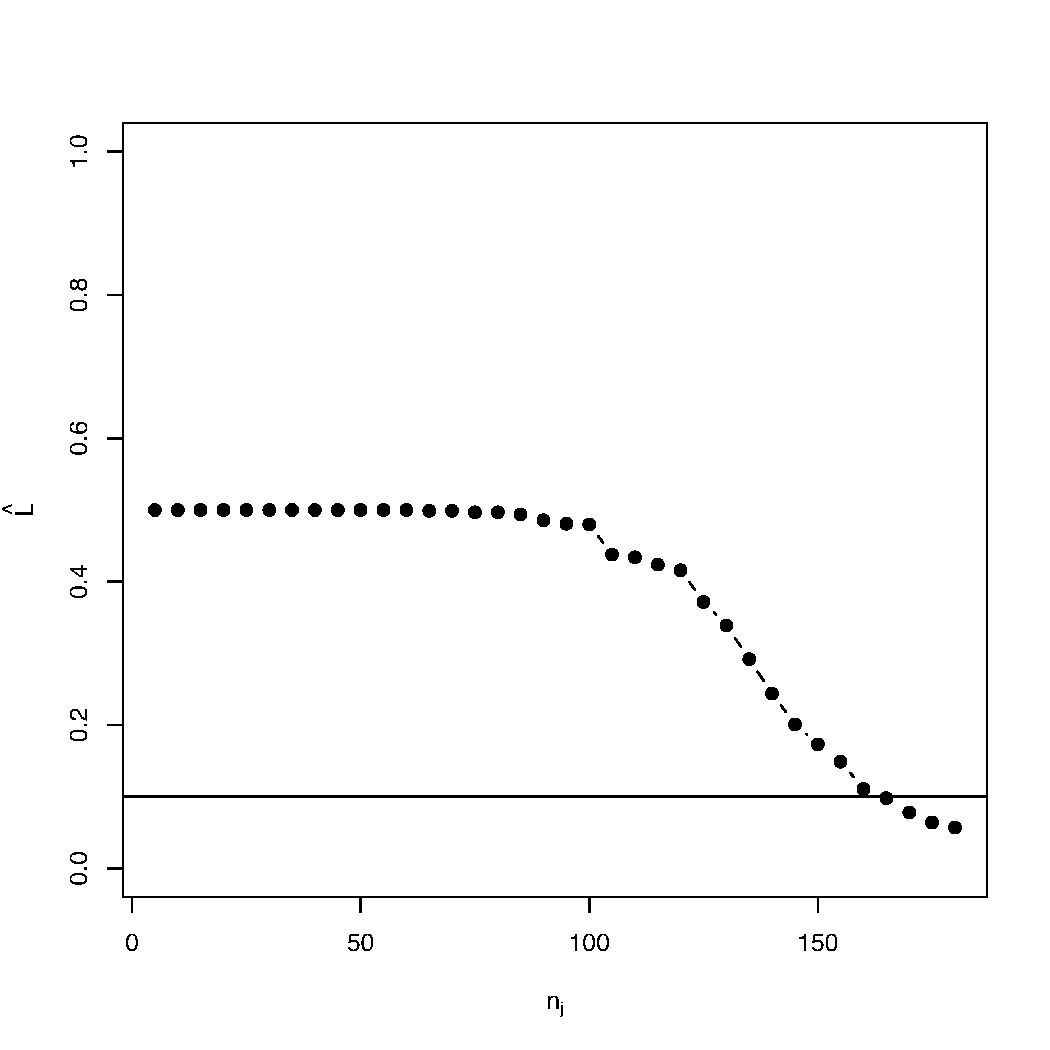
\includegraphics[width=.5\linewidth]{Lhatplot}
\caption{C.~elegans graph classification simulation results.  $\hL$  (the misclassification rate estimated upon with $1000$ testing samples) %$\hL^{1000}_{\PP}(g_{\mt{n}})$ 
is plotted as a function of class-conditional training sample size $n_j=\mt{n}/2$, suggesting that for $\varepsilon=0.1$ we can determine that $\MeB$ holds with $99\%$ confidence with just a few hundred training samples generated from $\PP[M,B]$. Each dot depicts an estimate for $L_{\PP}(g_{\mt{n}})$; standard errors are $(L_{\PP}(g_{\mt{n}})(1-L_{\PP}(g_{\mt{n}}))/1000)^{1/2}$\tr{; e}.g., $n_j = 180$; $k_n = 53$; $\hL^{1000}_{F}(g_{\mt{n}}) = 0.057$; standard error less than 0.01. We reject $H_0: L_{\PP}(g^*) \geq 0.10$ at $\alpha=0.01$. $L_{\PP}(g^*) \approx 0$ for this simulation.}
\label{fig1}
\end{figure}

Importantly, conducting this experiment {\it in actu} is not beyond current technological limitations. 3D superresolution imaging \cite{VaziriShank08} combined with neurite tracing algorithms \cite{HelmstaedterDenk08,Mishchenko09,LuLichtman09} allow the collection of a C. elegans brain-graph within a day. Genetic manipulations, laser ablations, and training paradigms can each be used to obtain a non-wild type population for use as $M=m_1$ \cite{deBonoMaricq05}, and the class of each organism ($m_0$ vs.~$m_1$) can also be determined automatically \cite{BuckinghamSattelle08}.


\bibliography{/Users/jovo/Research/latex/biblist}
\bibliographystyle{nature}



\end{document}

